  \section{Symulacje Numeryczne}
  
  
  \subsection{Oprogramowanie}

  Do oprogramowania symulacji wybrałem język Java, jako oferujący dobrą wydajność w obliczeniach numerycznych, z dojrzałym ekosystemem narzędzi i bibliotek oraz wieloplatformowy. Oskryptowanie zestawów symulacji (''przemiatanie'' po parametrach, wiele powtórzeń dla uśrednienia wyników) napisałem w języku Groovy.
  
  Kod źródłowy jest dostępny jako open-source, na licencji MIT, i dostępny w serwisie GitHub pod adresem http://github.com/tomash/fhneurotic .

  \subsubsection{Obliczanie Widma Mocy}

  Widmo mocy obliczane było z użyciem biblioteki JTransforms, używając szybkiej transformaty Fouriera (FFT). Ponieważ dane wejściowe, tj. wartości potencjału $v$ w zależności od czasu, były rzeczywiste, zastosowana była jednowymiarowa szybka transformata Fouriera dla danych rzeczywistych, zgodna z kanonicznym wzorem

  \begin{equation}
    F_k = \sum\limits^{N-1}_{n=0} v_n e^{-i2\pi \frac{k}{N} n}
  \end{equation}

  ale algorytm liczył pół elementów rzeczywistej transformaty, ponieważ druga połowa spełniała warunek symetrii

  \begin{equation}
    F_{N-k} = X^{*}_{k}
  \end{equation}

  Biblioteka JTransforms do liczenia FFT danych rzeczywistych stosuje algorytmy Split-Radix oraz Mixed-Radix. Dla optymalizacji liczenia FFT, ilość kroków symulacji (wartości $v$ poddawanych transformacie) w symulacjach jest potęgą 2.

  Widmo mocy (widmowa gęstość energii?) było obliczane zgodnie z kanoniczną postacią, jako kwadrat modułu  transformaty Fouriera

  \begin{equation}
    S_k = |F_k|^2
  \end{equation}

  $F_k$, a więc i tym samym $S_k$, nie były normalizowane dalszych w obliczeniach.

  \subsubsection{Obliczanie Signal-to-Noise Ratio}

  Stosunek sygnał-szum obliczałem poprzez podzielenie wartości lokalnie najwyższej (tj. piku głównego) przez średnią 10 wartości sąsiadujących (5 niższych, 5 wyższych).

  \begin{equation}
    SNR = \frac{P_i}{\frac{1}{10} \left ( \sum\limits^{i-1}_{j=i-5} P_j + \sum\limits^{i+5}_{j=i+1} P_j \right )}
  \end{equation}

  \subsection{Parametry symulacji}
  \label{sec:parametry}

  Punktem wyjścia do symulacji była praca A. Longtin \cite{longtin}, włączając w to znalezione przez niego optymalne zestawy parametrów pozwalające zaobserwować rezonans stochastyczny w rezonatorze FHN. Parametry symulacji, jeśli nie podano inaczej, są następujące:

  \begin{itemize}
    \item krok czasowy $\Delta t = 1/256 [s]$
    \item czas korelacji szumu $t_c = 0.01 [s]$
    \item okres sygnału periodycznego $q=1.0 [s]$ (częstotliwość $f=q^{-1}=1.0 [\frac{1}{s}]$)
    \item skalowanie czasu zmiennej v $\epsilon = 0.005$
    \item amplituda sygnału periodycznego $r=0.08$
    \item stała relaksacji $b=0.12$
    \item $a$ z równania \ref{eq:v} $a=0.5$
  \end{itemize}

  \subsection{Pojedynczy Neuron}
  
  Przed przystąpieniem do rozwiązywania układów wieloneuronowych rozpocząłem symulacje od zbadania pojedynczego neuronu, jak opisywany w pracy A. Longtin \cite{longtin}. Dzięki temu mogłem sprawdzić zarówno poprawność własnego oprogramowania, jak i model oraz zestaw parametrów opisane w wyżej wymienionej publikacji.
  
  Stochastyczne równania różniczkowe składające się na szum Ornsteina-Uhlenbecka całkowałem według metody opisanej w pracy Mannella, Palleschi \cite{mannella}. Po rozwiązaniu przedstawionego tam równania, szumu $\eta (t)$ liczony był następująco:

  \begin{equation} \label{eq:deta:final}
    \Delta \eta(t) = \Delta t(\lambda \xi_1(t) - \lambda \eta(t)) + \lambda \xi_2(t) \sqrt{\Delta t}
  \end{equation}

  \begin{equation} \label{eq:eta:final}
    \eta(t) = \eta(t-1) + \Delta \eta(t)
  \end{equation}

  Gdzie $\xi_1(t)$, $\xi_2(t)$ to dwa niezależne szumy gaussowskie w chwili t.
  
  Wyniki symulacji dla pojedynczego neuronu, z zestawem parametrów jak w \cite{longtin}, przedstawiają rysunki \ref{graphics:sym1v} (przebieg czasowy) i \ref{graphics:sym1fft} (widmo mocy).

  
  \begin{figure}
    \begin{center}
      \begin{tabular}{cc}
        \resizebox{100mm}{!}{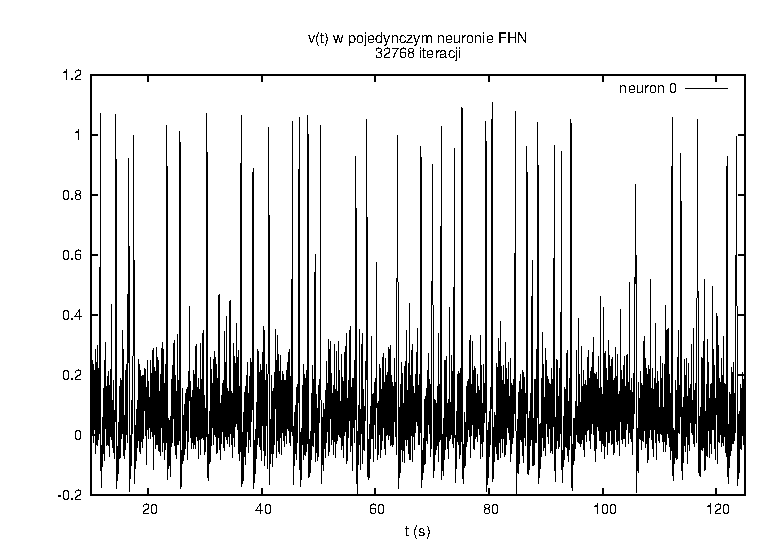
\includegraphics[width=140mm]{images/1neuron/1}} \\
        \resizebox{100mm}{!}{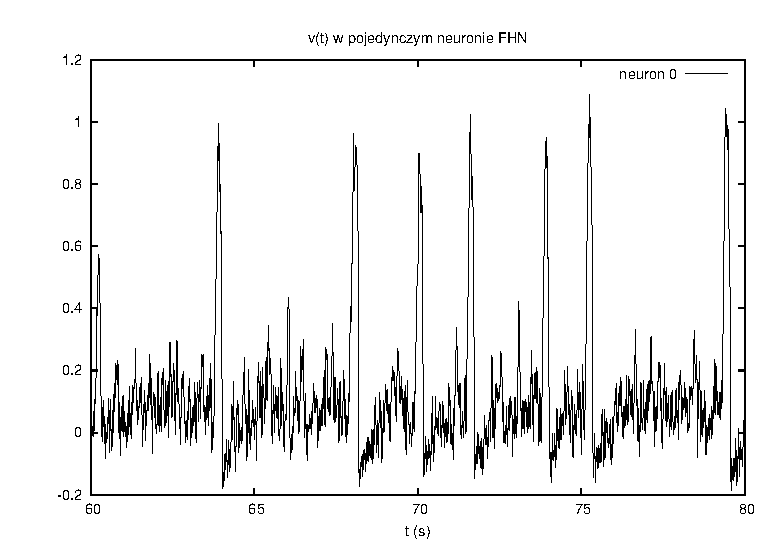
\includegraphics[width=140mm]{images/1neuron/2}} \\
      \end{tabular}
      \caption{Odtworzenie wyników Longtina. 32768 kroków iteracji, $D=1E{-5}$, pozostałe parametry według \ref{sec:parametry}}
      \label{graphics:sym1v}
    \end{center}
  \end{figure}

  Jest to przebieg zgodny z zaobserwowanym w pracy A. Longtin.

  \begin{figure}
    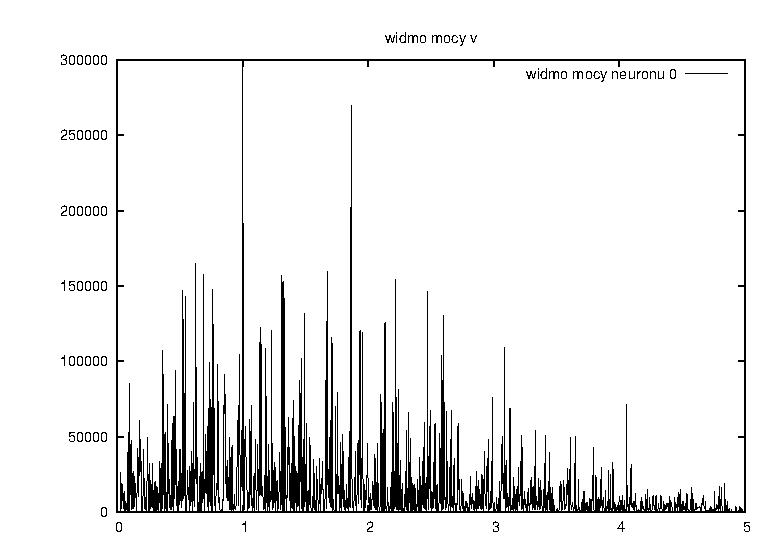
\includegraphics[width=140mm]{images/1neuron/3}
    \caption{Odtworzenie wyników Longtina: widmo mocy. Widać wyraźne piki dla częstotliwości podstawowej i jej wielokrotności. Dla piku głównego SNR = 8.26.}
    \label{graphics:sym1fft}
  \end{figure}

  
  \subsection{Układy Neuronów Bez Opóźnienia}
  \label{sec:uklad_bez_opoznienia}

  \subsubsection{Metodologia}
  
  Następnym krokiem pracy było połączenie neuronów (początkowo dwóch) w łańcuch, z sygnałem przekazywanym w jedną stronę, tzn. sygnał z neuronu $i$ jest odbierany przez neuron $i-1$ (neuron o indeksie 0 nie przekazuje swojego sygnału dalej, neuron o najwyższym indeksie nie odbiera sygnału od sąsiada). Opóźnienie w transmisji są na tym etapie zerowe. Te założenia prowadzą do następującej postaci równania \ref{eq:vext1}:

  \begin{equation} \label{eq:vext2}
    v_{i ext}(t) = \widetilde{v_{i+1}}(t)
  \end{equation}

  Neurony w układzie działały według równania zaproponowanego w rozdziale ~\ref{sec:przesuniecie_fazy}, bez opóźnienia (czyli $\tau_{n} = 0$).

  Ważnym elementem tego etapu badań było dobranie nowej wartości skalowania szumu D. Dotychczasowa wartość, czyli 1E-5, powodowała maksymalizację SNR w pojedynczym neuronie, ale w macierzach neuronów powoduje tłumienie wpływu sygnałów odebranych od połączonych neuronów (przesterowanie).

  Po wielu symulacjach z różnymi zakresami parametrów (patrz też wykres \ref{fig:graphics:snr_c_d_3d}) ustaliłem wartość D w okolicach $D=5E{-6}$ jako pozwalającą zaobserwować SR w pojedynczym neuronie jak i obserwować wyraźne zwiększanie SNR w wyniku odbierania sygnału od połączonych neuronów. Dla potwierdzenia tej hipotezy dalsze symulacje prowadzone były dla wartości D w zakresie od $D=1E{-6}$ do $D=2E{-5}$. 

  Ważna jest też czułość na sygnał odebrany od połączonego neuronu. Modelu FHN ma dynamikę bardzo podatną na zmiany parametrów, nawet w wąskich zakresach. W pracy Longtina dobrano optymalną amplitudę sygnału periodycznego $r=0.08$. Jest to wartość bardzo wysoka, gwarantująca silnie periodyczne zachowanie pojedynczego neuronu (dla wartości szumu z zakresu $5E{-6} - 5E{-5}$), podczas kiedy jest ono dość periodyczne już dla $r=0.05$. Suma amplitudy sygnału periodycznego i amplitudy sygnału odbieranego od sąsiednich neuronów powinna nie przekraczać maksymalnej użytecznej amplitudy pojedynczego neuronu $r_{max}=0.08$.
  
  Po wielu próbach wybrano amplitudę $r=0.05$ i czułość $s=0.02$, jako pozwalające uzyskać wyraźny wpływ połączonych neuronów, a jednocześnie zwiększać SNR w kolejnych neuronach łańcucha bez wysycenia na drugim-trzecim neuronie.

  \subsubsection{Łańcuch 9 neuronów}

  Wynik symulacji po uwzględnieniu ww. eksperymentów przedstawia rysunek \ref{fig:graphics:sim:2010_12_07_01}, z bardziej czytelnym przecięciem płaszczyznami $n=0$ i $n=8$ na rysunku \ref{fig:graphics:sim:2010_12_07_02}.

  \begin{figure}
    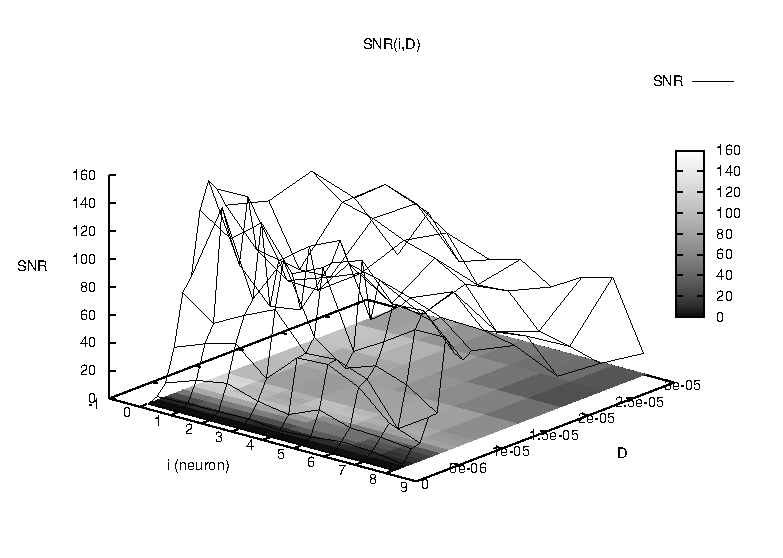
\includegraphics[width=140mm]{images/9neuron/2010_12_07_01}
    \caption{Układ 9 neuronów bez opóźnienia. Widać wyraźny wzrost SNR zgodnie z ''kierunkiem'' przekazywania sygnału. $r=0.05$, $s=0.02$, SNR liczony na podstawie nienormalizowanego widma mocy. 65536 ($2^{16}$) kroków iteracji (256 okresów) dla każdego zestawu parametrów. Wartości SNR uśrednione, po 20 pełnych symulacji dla każdej wartości D.}
    \label{fig:graphics:sim:2010_12_07_01}
  \end{figure}

  \begin{figure}
    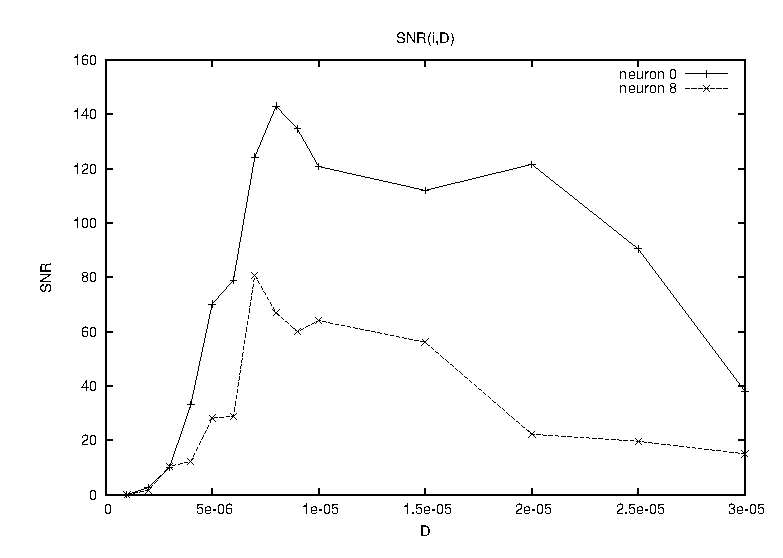
\includegraphics[width=140mm]{images/9neuron/2010_12_07_02}
    \caption{Przecięcie wyników z rysunku \ref{fig:graphics:sim:2010_12_07_01} płaszczyznami $n=0$ (maksima SNR w neuronie odbierającym sygnał na końcu) i $n=8$ (maksima SNR w neuronie nieodbierającym sygnału)}
    \label{fig:graphics:sim:2010_12_07_02}
  \end{figure}

  Zaobserwowane przebiegi czasowe były zgodne ze spodziewanym analitycznie wynikiem: z każdym kolejnym neuronem w łańcuchu następował wzrost SNR (do wartości granicznej około 200) ze względu na wzrost prawdopodobieństwa wzbudzenia w przypadku wzbudzenia neuronu sąsiedniego.



  Następnym krokiem było wprowadzenie do układu rozciągłości przestrzennej, czyli różnic w fazach sygnału periodycznego odbieranego przez poszczególne neurony, na tym etapie bez opóźnień transmisji. Aby uzyskać maksymalny efekt antysynchronizacji, wybrano różnicę faz pomiędzy sąsiadującymi rezonatorami równą $\Delta \phi_{i,i+1} = \pi $ . Oczekiwanym skutkiem było gwałtowne obniżenie SNR we wszystkich neuronach z wyjątkiem ostatniego (jako że nie odbiera on sygnału od sąsiadujących). Wyniki przedstawia rysunek \ref{fig:graphics:sim:2010_12_06_01}.

  \begin{figure}
    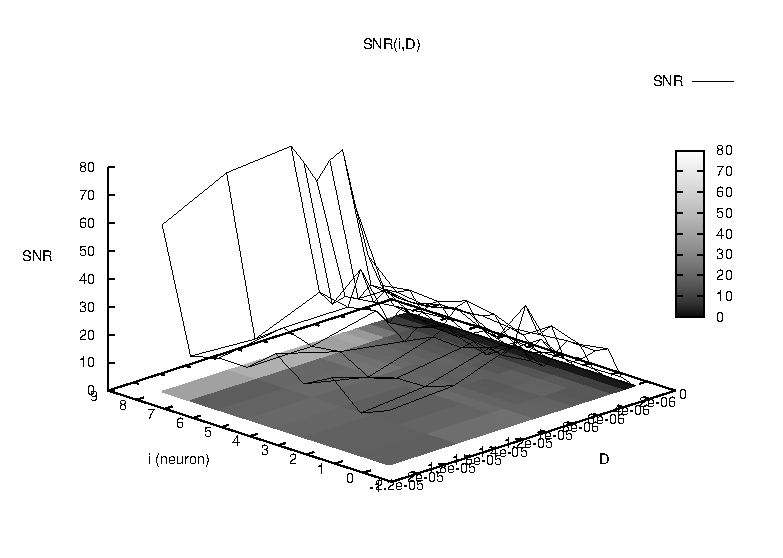
\includegraphics[width=140mm]{images/9neuron/2010_12_06_01}
    \caption{Układ 9 neuronów bez opóźnienia, z różnicą faz $\Delta \phi_{i,i+1} = \pi $. Widać, że dla neuronów które odbierały sygnał od sąsiada SNR utrzymuje się na bardzo niskim poziomie, o wiele niższym od neuronu nieodbierającego sygnału (neuron ósmy). Parametry jak w symulacjach przedstawionych na rys. \ref{fig:graphics:sim:2010_12_07_01}}
    \label{fig:graphics:sim:2010_12_06_01}
  \end{figure}


  \subsection{Układy neuronów z opóźnieniem}

  \subsubsection{Metodologia}
  
  Do układu opisanego powyżej dodałem opóźnienie w przekazywaniu sygnałów, w sposób opisany w rozdziale ~\ref{sec:przesuniecie_fazy}. Budując łańcuch dokładnie taki jak, zbudowałem łańcuch z opóźnieniem transmisji. Opóźnienie pomiędzy każdą parą sąsiadujących neuronów jest wspólne dla wszystkich par i wynosi $\tau$. To założenia prowadzi do następującej postaci równania \ref{eq:vext2}:

  \begin{equation} \label{eq:vext3}
    v_{i ext}(t) = \widetilde{v_{i+1}}(t-\tau)
  \end{equation}

  Mając gotowy model wykonane zostały symulacje macierzy złożonych z 2. i 9. rezonatorów.

  
  \subsubsection{Łańcuch 2 neuronów}

  Pierwszym krokiem w badaniu macierzy neuronów z opóźnieniem uczyniłem zbadanie macierzy dwuelementowej, celem znalezienia zależności pomiędzy podstawowymi parametrami symulacji.

  Przez c oznaczyłem opóźnienie transmisji, jako wielokrotność okresu sygnału periodycznego. Przesunięcie fazowe sygnału periodycznego p wynosiło pół okresu.
  Znaleziona zależność SNR (WYKRES) od c oraz D (skalowanie szumu) posiada bardzo wyraźną ''grań'' dla c=0.5, co potwierdza oczekiwania: maksymalizację SNR można osiągnąć poprzez kompensację przesunięcia fazowego (rozciągłości przestrzennej) identycznym (lub prawie identycznym) opóźnieniem w transmisji.

  \begin{figure}
    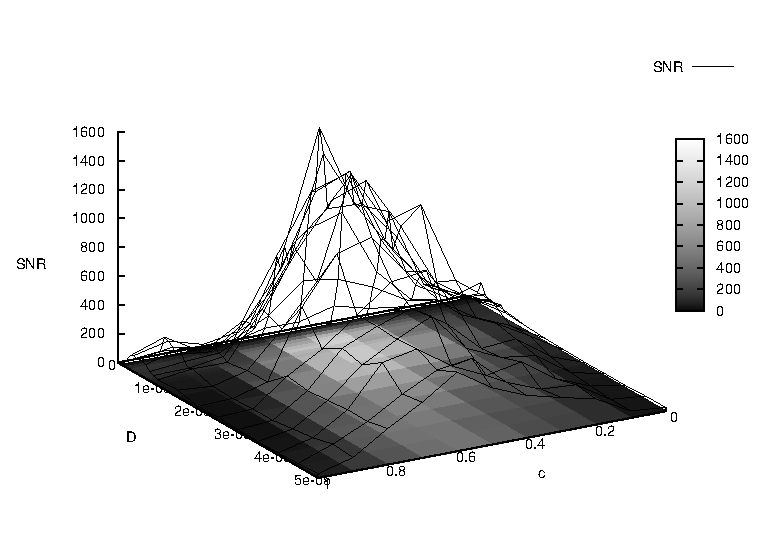
\includegraphics[width=140mm]{images/2neuron/3d}
    \caption{Dwa neurony, SNR w ''odbierającym'' w zależności od opóźnienia w transmisji c (jako wielokrotność T), dla przesunięcia fazowego równego 0.5T. Widać wyraźną ''grań'' kiedy c = p (= 0.5T)}
    \label{fig:graphics:snr_c_d_3d}
  \end{figure}

  Wyniki dla dwóch neuronów potwierdzają hipotezę. Jednakże dla analizy relacji skalowania symulowana była także macierz 9 neuronów z opóźnieniem transmisji.

  \subsubsection{Łańcuch 9 neuronów z opóźnieniem}


  Wpierw zostały zbadane łańcuchy neuronów FHN połączonych tak, aby opóźnienie transmisji kompensowało rozciągłość przestrzenną, czyli $c = \Delta \phi$. Takie łańcuchy powinny dawać wyniki zbliżone do układu o tej samej strukturze, ale bez opóźnień i przesunięć fazowych, jak przedstawione w rozdziale \ref{sec:uklad_bez_opoznienia}.
    
  %Po dołożeniu opóźnień po zbudowaniu jednokierunkowego łańcucha jak w rozdziale \ref{sec:uklad_bez_opoznienia} wykonano jego symulacje. Wyniki zamieszczono na rysunkach \ref{fig:graphics:sim:2010_12_07_02}

  \begin{figure}
    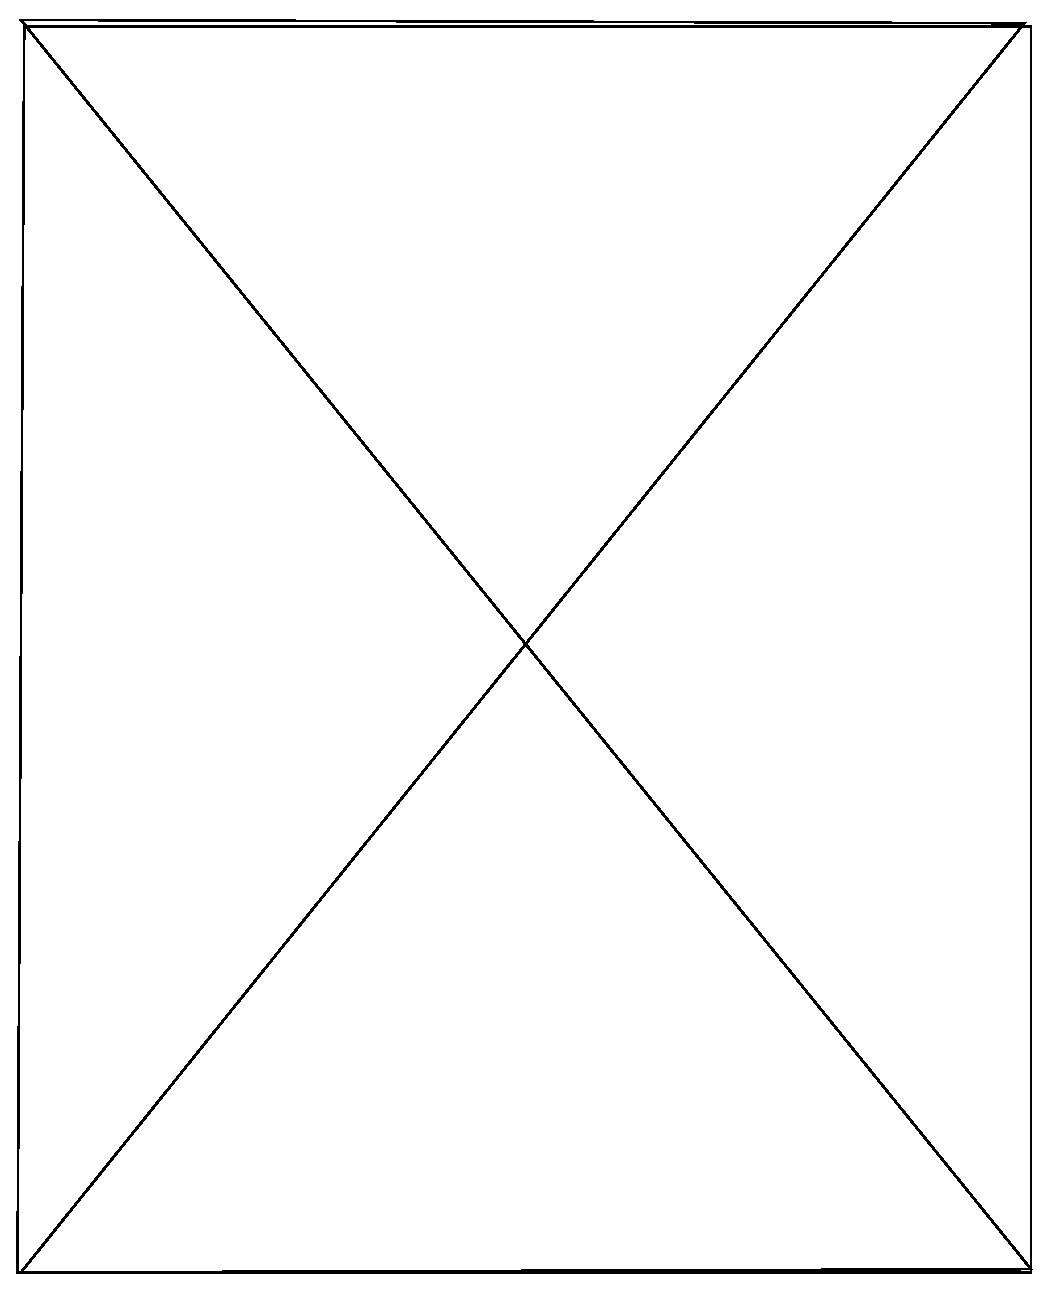
\includegraphics[width=140mm]{images/pending}
    \caption{Układ 9 neuronów rozciągły przestrzennie o przesunięciu fazowym $\phi_i = 0.111 T i, \Delta \phi = 0.111 T$ i z opóźnieniem transmisji dobranym do kompensowania rozciągłości przestrzennej $c = \Delta \phi$. Wzrost SNR zgodnie z ''kierunkiem'' przekazywania sygnału jest maksymalny, do wartości granicznej około 1600. SNR liczony na podstawie nienormalizowanego widma mocy. 65536 ($2^{16}$) kroków iteracji (256 okresów) dla każdego zestawu parametrów.}
    \label{fig:graphics:sim:2010_10_03}
  \end{figure}

  Wyniki, przedstawione na rysunku \ref{fig:graphics:sim:2010_10_03}, są zgodne z oczekiwaniami: przestrzennie rozciągły łańcuch neuronów z opóźnieniami transmisji kompensującymi różnice fazowe [docierającej fali] w istocie zachowuje się jak analogiczny układ pozbawiony opóźnień i różnic fazowych.

  Na rysunku \ref{fig:graphics:sim:2010_10_03} można zaobserwować ciekawe, omówione w rozdziale \ref{sec:uklad_bez_opoznienia} zjawisko. Otóż po osiągnięciu przez neuron i-ty regularności bliskiej maksymalnej ($SNR \approx 200$ dla $2^{16}$ iteracji), w neuronie i-1, do którego przekazywany jest sygnał, następował wyraźny spadek SNR. Wynika z tego, że zbyt mocny nieszumowy sygnał wejściowy może przesterowywać neuron i tym samym wywoływać suboptymalny SR.


